\documentclass[conference]{IEEEtran}

\usepackage[T1]{fontenc}
\usepackage[utf8]{inputenc}
\usepackage{graphicx}
\usepackage{cite}
\usepackage{amsmath,amssymb}
\usepackage{booktabs}
\usepackage{array}
\usepackage{float}
\usepackage{hyperref}
\usepackage{xcolor}
\usepackage{url}

\graphicspath{{./}}

\emergencystretch=2em

\hypersetup{
  colorlinks=true,
  linkcolor=black,
  citecolor=black,
  urlcolor=blue
}

\title{DEMO: From Natural Language to Live 5G API Calls ---
A CAPIF-Compliant, Multi-LLM Intent Orchestration Platform}

\author{
  \IEEEauthorblockN{T\"{u}rkan Do\u{g}a Durak$^{\ast}$,\; Engin Zeydan$^{\ddag}$,\; Luis Blanco$^{\ddag}$}\\
  \IEEEauthorblockA{%
    $^{\ast}$Software Engineering Department,
    Manisa Celal Bayar University, Manisa, T\"{u}rkiye, 45400.\\
    $^{\ddag}$Centre Tecnol\`{o}gic de Telecomunicacions de Catalunya
    (CTTC/CERCA), Castelldefels, Spain, 08860.\\
    Email: turkandogadurak@hotmail.com,\; \{ezeydan, luis.blanco\}@cttc.es
  }
}

\begin{document}
\maketitle

\begin{abstract}
In this paper, we demonstrate a working, open-source telco orchestration platform that
converts free-text operator intents into live 5G API calls in under
three seconds.
Demo users can submit requests, watch a
two-phase large-language-model (LLM) planner route them to the correct CAMARA service and
construct a standards-compliant payload, then observe a three-layer
deterministic validator clear every constraint tier before the call is
forwarded to a live, 3GPP CAPIF-registered provider.
Switching LLM backends, GPT-4o-mini, Claude\,Haiku\,4.5, and
Gemini\,2.5\,Flash, requires no code changes; structurally identical
payloads from all three confirm provider-agnostic schema grounding.
A 300-entry ground-truth evaluation shows all LLM modes
achieve an Intent-to-API Workflow Success Rate (IWSR)\,$>$\,94.7\,\%,
outperforming the keyword-based deterministic baseline (IWSR\,=\,83.3\,\%)
on diverse phrasings.
All source code, datasets, and evaluation scripts are available at
\url{https://github.com/doadurak/mini-telco-platform}; a narrated
demo video is available online~\cite{demo_video2025}.
\end{abstract}

\begin{IEEEkeywords}
CAPIF, CAMARA, intent-based networking, LLM orchestration,
5G API exposure, live demonstration, zero-touch automation
\end{IEEEkeywords}


\section{Introduction and Motivation}

Zero-touch network management for Beyond-5G and 6G demands
orchestration layers that accept high-level operator intents and
translate them into precise, standards-compliant API invocations
without manual payload composition~\cite{coronado2022}.
3GPP CAPIF (TS\,23.222)~\cite{3gpp_capif} and the GSMA CAMARA
project~\cite{camara2022} define the governance and semantic
specifications enabling vertical industries to consume network
capabilities through standardised APIs.
Closing the intent-to-API gap in a \emph{live} deployment remains
largely unsolved.

\textbf{Related work and novelty.}\;
OpenCAPIF~\cite{molina2022} and similar CAPIF experimentation
platforms focus on exposure infrastructure but provide no
natural-language planning layer.
Turkovic~et~al.~\cite{turkovic2025} demonstrated live CAMARA\,QoD
integration (230--340\,ms) but relied on manual payload construction.
Maatouk~et~al.~\cite{maatouk2025} identified hallucination as the key
risk in telecom LLM deployments, and Liu~et~al.~\cite{liu2024} showed
that ungrounded GPT-4 achieves only 40\,\% compliance on JSON-schema
tasks.
To the best of our knowledge, no prior openly available platform
simultaneously addresses live CAPIF invoker onboarding,
multi-provider CAMARA execution, schema-grounded LLM planning, and
a three-layer deterministic validator, with every component
operating live: Public Key Infrastructure (PKI)-issued CAPIF certificates, containerised CAMARA
providers, and production LLM API calls that attendees trigger
themselves.


\section{Platform Architecture}
\label{sec:arch}


\begin{figure*}[t]
  \centering
  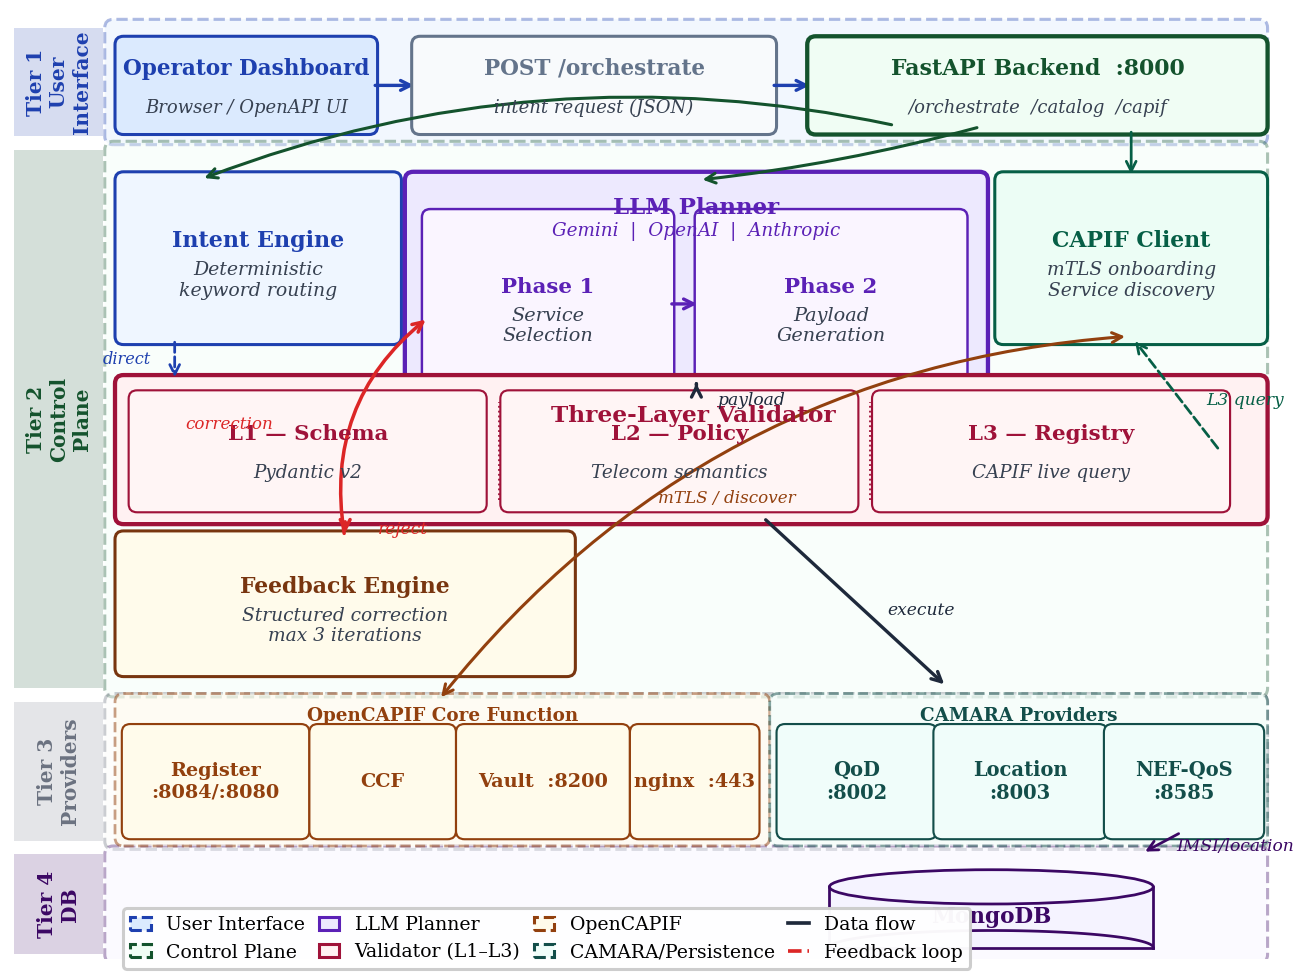
\includegraphics[width=0.82\textwidth]{nof_fig1_arch.png}
  \caption{Four-tier platform architecture.
  On startup, the CAPIF\,Client (CAPIF-2e) generates an RSA-2048 key
  pair, submits a Certificate Signing Request (CSR) to the OpenCAPIF Register service~\cite{molina2022}
  backed by HashiCorp Vault PKI, and receives a signed certificate and
  \texttt{apiInvokerId}.
  All subsequent provider discovery and invocation use mutual TLS (mTLS).
  Every LLM-generated payload is intercepted by the three-layer
  validator (L1--L3) before any CAMARA provider call is made.}
  \label{fig:arch}
\end{figure*}

The platform comprises nine components across four logical tiers
(Fig.~\ref{fig:arch}).
The \emph{interface tier} provides an operator web dashboard and a
FastAPI backend at port\,8000 exposing a single
\texttt{POST\,/orchestrate} endpoint.
The \emph{control-plane tier} houses an Intent Engine, a two-phase
LLM\,Planner, a three-layer Validator, a Feedback Engine (up to
three correction iterations), and a CAPIF\,Client.
The \emph{provider tier} delivers four CAMARA-standardised services,
QoD\,v1.1.0, QoS\,Profiles, QoS\,Provisioning
(3GPP\,TS\,29.122), and Location\,Retrieval\,v0.5, registered
through the API Exposing Function (AEF) via the CAPIF-4 reference
point, with provider domain onboarding (CAPIF-5) completed at
stack initialisation.
A \emph{persistence tier} (MongoDB) logs every intent, validator
verdict, latency, and provider response.

The \emph{Orchestration Engine} and \emph{Validation Layer} visible
in Fig.~\ref{fig:arch} implement the two-phase LLM planner and
three-layer validator, respectively:

\textit{Two-Phase LLM Planner:}\;
Phase\,1 selects the correct CAMARA service and operation by reasoning
over a schema-grounded summary of all registered APIs, optionally
consulting the live CAPIF discovery endpoint.
Phase\,2 generates the full JSON payload by injecting the complete
OpenAPI schema for the selected operation as system context, the
grounding step that achieves Schema Compliance Rate (SCR) and Semantic Validity Rate (SVR) above 97\,\% across all
tested providers, confirming schema-grounded planning as a reliability
mechanism~\cite{flowmind2023}.
A pluggable dispatcher routes to GPT-4o-mini, Claude\,Haiku\,4.5, or
Gemini\,2.5\,Flash at runtime with no code changes.

\textit{Three-Layer Validator:}\;
\textit{L1} enforces Pydantic\,v2 schema, types, and field constraints
(SCR).
\textit{L2} applies eight telecom-semantic rules: E.164 phone format,
enumerated QoS profile membership, session duration in $[1,7200]$\,s,
and unicast IPv4 address (SVR).
\textit{L3} queries the live CAPIF registry to confirm the requested
service identifier exists (Hallucination Rate, HR).
On failure at any layer, the Feedback Engine sends a structured,
layer-tagged correction prompt and retries up to three times.
This separation of probabilistic LLM reasoning from deterministic
constraint enforcement is the mechanism that enables quantified
reliability guarantees~\cite{flowmind2023}.


\section{Live Demonstration}
\label{sec:demo}


\begin{figure}[t]
  \centering
  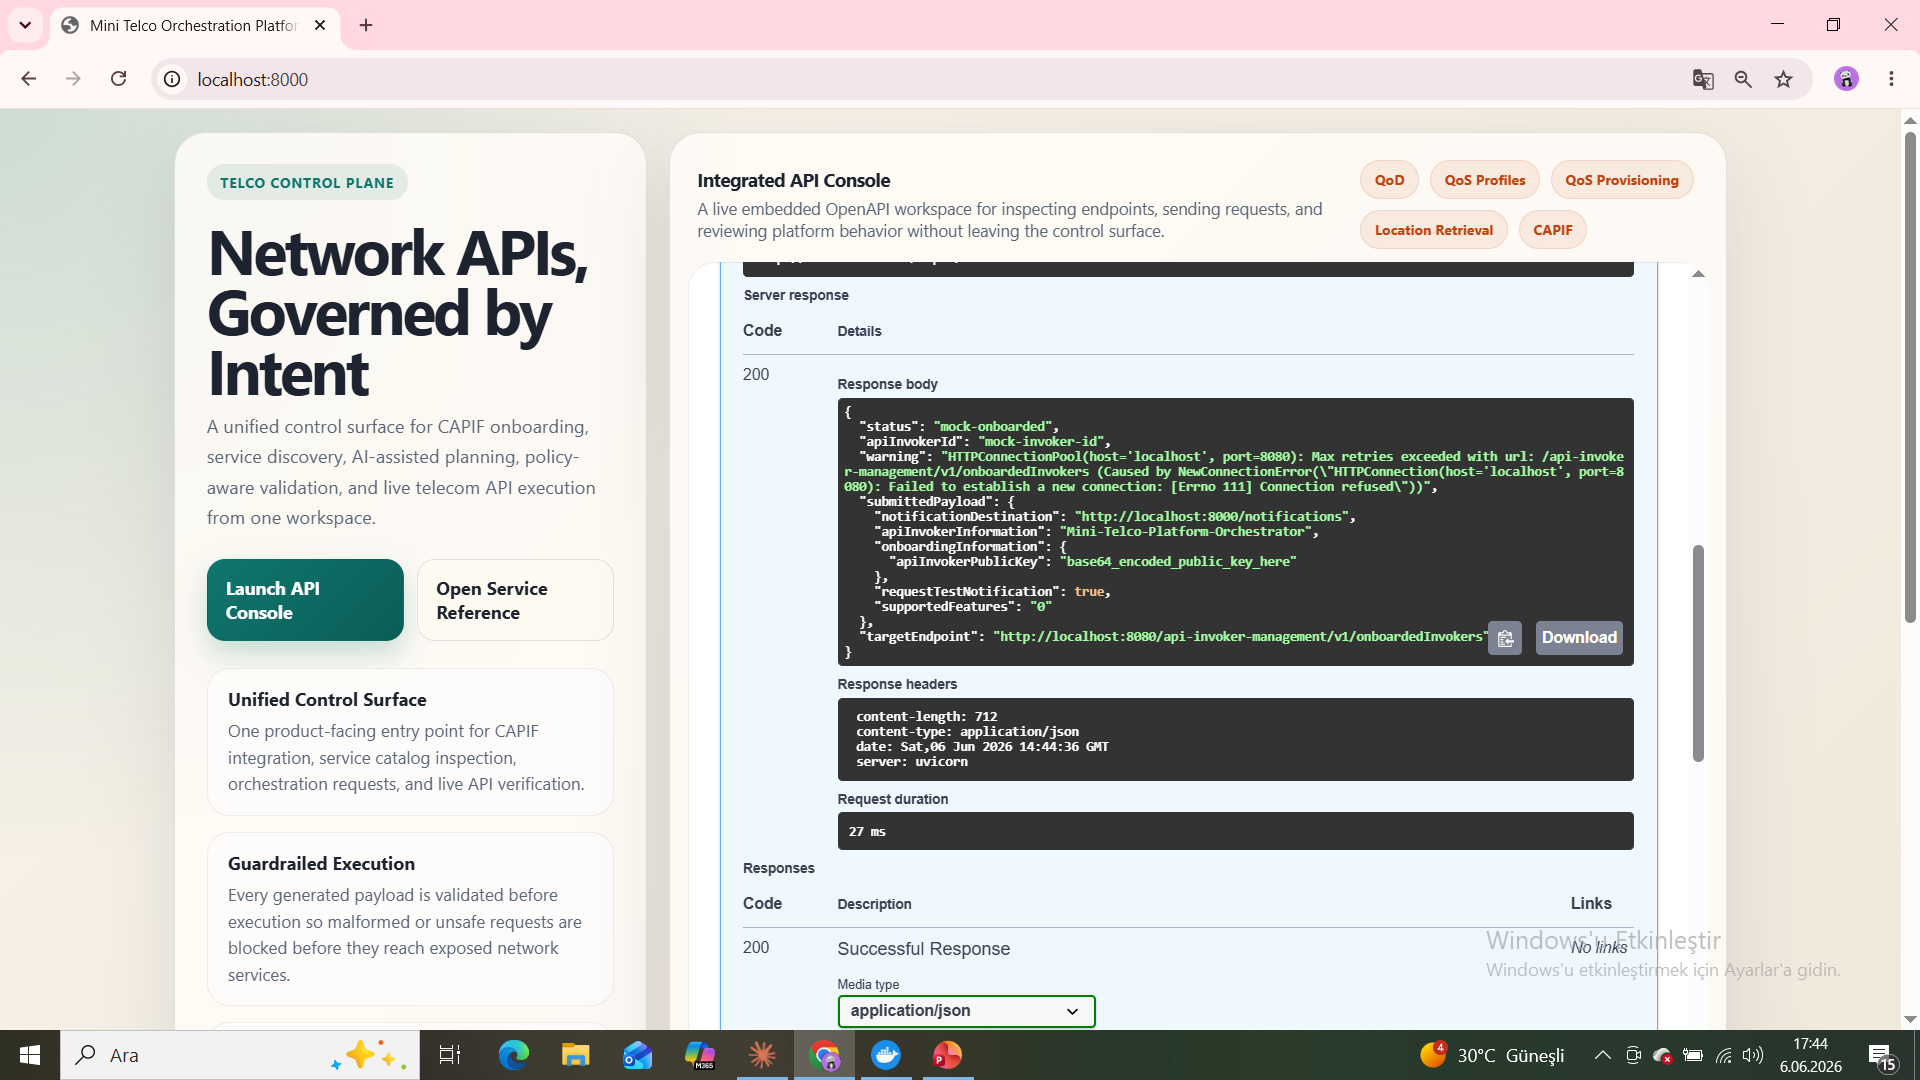
\includegraphics[width=\columnwidth]{system1}
  \caption{Live \texttt{POST\,/orchestrate} response in the platform UI.
  The Orchestration panel shows the free-text intent (top),
  the LLM-selected CAMARA service and schema-grounded payload (middle),
  and the provider HTTP response with status code and latency (bottom).
  Per-layer validator outcomes (L1\,SCR, L2\,SVR, L3\,HR) appear
  inline before the CAMARA provider call is made.}
  \label{fig:ui}
\end{figure}

The demo runs on a single conference laptop with all CAPIF and CAMARA
infrastructure containerised; the only external dependencies are three
LLM API keys.
The operator control panel (Fig.~\ref{fig:ui}) displays, in one
browser tab, the intent typed, the CAMARA service selected, the
schema-grounded payload, per-layer validator outcomes (L1/L2/L3), and
the live provider HTTP response, all within $\approx$\,3\,s.
The Catalog module lets attendees confirm that the service the LLM
selected is registered in the live CAPIF registry.

\subsection[Scenario 1 --- English QoD Intent]{Scenario\,1 --- QoD Session Intent}

The attendee types:
\begin{quote}\small
\textit{``Activate video-streaming quality for +905321234567
for the next 30\,minutes.''}
\end{quote}
Phase\,1 routes to \path{qod-sessions/createSession};
Phase\,2 generates \texttt{QOS\_E\_STREAMING} /
\texttt{duration\,=\,1800\,s}.
All three validator layers pass; the QoD provider returns HTTP\,201
with a \texttt{sessionId} and \texttt{status:\,REQUESTED} in
$\approx$\,3\,s.

\subsection[Scenario 2 --- Location Retrieval]{Scenario\,2 --- Location Retrieval}

The attendee types:
\begin{quote}\small
\textit{``Retrieve the current location of device +905551112233.''}
\end{quote}
Phase\,1 routes to \path{location-retrieval/retrieveLocation};
the provider returns WGS-84 coordinates with HTTP\,200.

\subsection[Scenario 3 --- Ambiguous Intent and Feedback Recovery]{Scenario\,3 --- Ambiguous Intent and Feedback Recovery}

The attendee types:
\begin{quote}\small
\textit{``Set the best possible network parameters for +12025550180
used for smart-grid telemetry.''}
\end{quote}
This phrasing straddles the QoD\,/\,QoS\,Provisioning boundary, a
hard case drawn from the 300-entry evaluation dataset.
Attendees observe either a clean Phase\,1 decision routing to
\path{qos-provisioning/provisionQoS}, or, if the LLM
misclassifies, the Feedback Engine emitting a layer-tagged
correction prompt and retrying, with every intermediate step visible
in the Orchestration panel.

\subsection[Scenario 4 --- Live Multi-LLM Backend Switch]{Scenario\,4 --- Live Multi-LLM Backend Switch}

The operator calls \texttt{POST\,/config/provider} to switch the
active LLM backend from \texttt{openai} to \texttt{anthropic} to
\texttt{gemini}, a live API call with no container restart or code
change.
Scenario\,1 is resubmitted after each switch.
Attendees observe structurally identical CAMARA payloads from three
independent LLM backends, with minor lexical variation only in
Phase\,1 chain-of-thought reasoning, confirming that the
schema-grounding mechanism, not the model, is the source of
reliability.


\section{Demonstration Apparatus}
\label{sec:apparatus}


\begin{table}[t]
\centering
\caption{Hardware and Software Configuration}
\label{tab:setup}
\small
\begin{tabular}{ll}
\toprule
\textbf{Component} & \textbf{Specification} \\
\midrule
Host OS            & Ubuntu\,22.04\,LTS (or Windows\,11\,+\,WSL\,2) \\
Container runtime  & Docker Engine\,26\,+\,Compose\,v2 \\
CAPIF stack        & OpenCAPIF (nginx, Vault\,PKI, MongoDB) \\
CAMARA providers   & 4 services, local Docker containers \\
LLM backends       & OpenAI, Anthropic, Google (live API keys) \\
Min.\ host         & 16\,GB RAM, 4-core CPU ($\approx$6\,GB peak) \\
\bottomrule
\end{tabular}
\end{table}

Table~\ref{tab:setup} lists the configuration.
The full stack starts with a single \texttt{docker compose up}; a
startup script completes CAPIF-2e invoker onboarding (RSA key pair,
CSR, certificate) and verifies all four CAMARA providers before
signalling readiness, cold-start under two minutes.
In the event of external LLM API unavailability, the system falls back
to deterministic mode, keeping the three-layer validation and CAPIF
pipeline demonstrable.
A narrated demo video is available online~\cite{demo_video2025}.

\begin{table}[t]
\centering
\caption{Reliability --- 300-Entry Ground-Truth Evaluation}
\label{tab:metrics}
\small
\setlength{\tabcolsep}{3.5pt}
\begin{tabular}{lrrrr}
\toprule
\textbf{Provider} & \textbf{IWSR} & \textbf{SCR} & \textbf{SVR} & \textbf{SS} \\
\midrule
Deterministic      & 83.3\,\% & 100.0\,\% & 100.0\,\% & 0.962 \\
GPT-4o-mini        & \textbf{95.7\,\%} & 98.3\,\% & 97.3\,\% & \textbf{0.973} \\
Claude\,Haiku\,4.5 & 94.7\,\% & \textbf{98.7\,\%} & \textbf{98.7\,\%} & 0.925 \\
Gemini\,2.5\,Flash & 94.7\,\% & 98.7\,\% & 97.0\,\% & 0.943 \\
\bottomrule
\end{tabular}
\vspace{2pt}

\noindent\footnotesize
IWSR\,=\,Intent-to-API Workflow Success Rate; SCR\,=\,Schema
Compliance; SVR\,=\,Semantic Validity; SS\,=\,Stability Score:
fraction of $k\!=\!3$ repeated runs yielding identical service
selection and a valid payload.
HR and RRF excluded for space; LLM-mode HR (2.3--4.0\,\%) and
RRF (28.6--60.0\,\%) are in the repository dataset.
Deterministic HR\,=\,16.7\,\%: intents outside the keyword vocabulary
rejected at L3 (not LLM hallucination).
Dataset: 8 E.164 country codes, 3 stratified difficulty tiers,
5 CAMARA service categories, coverage designed to stress Phase\,1
routing boundaries, not to optimise aggregate IWSR.
\end{table}

Table~\ref{tab:metrics} summarises offline reliability.
All LLM modes outperform the deterministic baseline on IWSR,
directly verifiable in Scenario\,4, confirming that schema
grounding compensates for LLM probabilism despite slightly lower SCR.
Stratified results show hard-difficulty intents drive most failures
(hard IWSR\,=\,87--94\,\% vs.\ 98--100\,\% at easy/medium),
consistent with the boundary cases in Scenarios\,3 and\,4.


\section{Conclusion}
\label{sec:conclusion}


We present an interactive demonstration of the first openly available
platform that combines live 3GPP CAPIF invoker onboarding,
multi-provider CAMARA service execution, schema-grounded multi-LLM
intent planning, and a three-layer deterministic validator.
Conference attendees submit natural-language intents and observe the
complete pipeline, from certificate
issuance and registry discovery to LLM reasoning, constraint
validation, and live API response, in real time, from a
fully reproducible single \texttt{docker compose up} deployment.


\bibliographystyle{IEEEtran}
\bibliography{references}

\end{document}
